\documentclass{standalone}
\usepackage{tikz}
\usetikzlibrary{plotmarks}
\begin{document}

\pgfmathsetmacro{\hilight}{0.6}
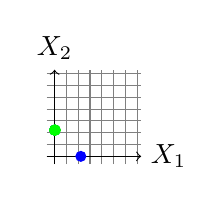
\begin{tikzpicture}[scale=1.0]
    \draw[gray,thin,step=0.15] (-0.1,-0.1) grid (1.1,1.1);
    \draw[->] (-0.1,0) -- (1.1,0) node[right] {$X_1$};
    \draw[->] (0,-0.1) -- (0,1.1) node[above] {$X_2$};

    \def\alpha{1/3}

    % First ladder (blue)
    \foreach[count=\i]\angle in {0,60,...,300}{
        \pgfmathsetmacro{\ang}{atan(\angle)}
        \pgfmathsetmacro{\angle}{mod(\ang,360)}
        \pgfmathsetmacro{\dang}{\angle-\alpha}
        \pgfmathsetmacro{\da}{mod(\dang,180)}
        \pgfmathsetmacro{\hilight}{ifthenelse(\da<90 || \da>270,\hilight,0)}
        \fill[blue!\hilight, opacity=1] (\angle:\alpha) circle[radius=2pt];
    }

    % Second ladder (green)
    \foreach[count=\i]\angle in {30,90,...,330}{
        \pgfmathsetmacro{\ang}{atan(\angle)}
        \pgfmathsetmacro{\angle}{mod(\ang,360)}
        \pgfmathsetmacro{\dang}{\angle-\alpha}
        \pgfmathsetmacro{\da}{mod(\dang,180)}
        \pgfmathsetmacro{\hilight}{ifthenelse(\da<90 || \da>270,\hilight,0)}
        \fill[green!\hilight, opacity=1] (\angle:\alpha) circle[radius=2pt];
    }
\end{tikzpicture}
\end{document}